\section{Motivating example}\label{sec:motivation}

Quadrivalent meningococcal conjugate vaccines are licensed on immunogenicity, and the confirmatory standard is a set of serogroup-specific binary endpoints that must all be met. Yang et al\cite{yang2024} describe a trial of a quadrivalent meningococcal tetanus toxoid-conjugate vaccine in which seroresponse for each of serogroups A, C, W and Y was a co-primary endpoint, success requiring non-inferiority to the licensed comparator on all four with a margin of $-10$ percentage points, and report comparator seroresponse rates of $0.425$, $0.497$, $0.448$ and $0.434$. Four binary endpoints in conjunction is exactly the setting in which the type II error of a co-primary analysis inflates and the sample size rises accordingly.

Upstream of such a trial sits a formulation-selection stage. {\O}stergaard et al\cite{ostergaard2009} compared five candidate MenACWY-TT formulations, differing in polysaccharide content and conjugation method, against a licensed ACWY polysaccharide vaccine in two open-label studies of 50 adults aged 18--25 and 125 adolescents aged 15--19, with the percentage of serum bactericidal antibody (rSBA) responders to each of serogroups A, C, W-135 and Y as the immunogenicity endpoints. Responder percentages did not differ from control for any formulation on any serogroup, with one exception: serogroup A was lower after one formulation. The selection problem is therefore $M=5$ candidates and $K=4$ binary components, $2^K=16$ response patterns per subject, and a concurrent control; and its outcome was, in effect, a judgement over four responder rates per formulation made on 25--35 subjects per arm.

Three features of this setting make it the natural home for the design proposed here. First, the components are positively dependent, since they are responses of the same immune system to conjugates of the same carrier, and a better formulation tends to be better on every serogroup; a scalar summary of the four responder rates therefore carries most of the information that distinguishes formulations, and a selection rule that applies the conjunctive criterion to each candidate discards it. Second, the components have a clinically meaningful weighting: serogroup-specific disease burden differs by age and region, so a weighted responder composite of the kind introduced by Zaslavsky\cite{zaslavsky2013} is interpretable and can be fixed from epidemiological data before the trial. Third, the development ran as a small open-label formulation study followed by separate confirmatory trials; a seamless design that randomises the candidates and control in stage 1, selects on the composite, continues the selected formulation and control into stage 2, and confirms on the four co-primary non-inferiority endpoints with the stage-1 data included, is the obvious alternative, and the question the paper answers is what it costs in error control and what it saves in sample size.

The same example supplies the design's principal caveat. The single-serogroup shortfall seen for one formulation is a failure on one component with adequate responses on the other three, and a composite that averages the four responder rates registers it weakly. Section~\ref{sec:e2e} quantifies this: the composite gate proceeds to stage 2 far more often than a conjunctive gate when one component is inert, and the error rate is protected only by the final co-primary test. Whether that cost is acceptable depends on how plausible single-serogroup failure is for the candidates at hand, and the design rule of Section~\ref{sec:e2e} places it in the scenario set for that reason.

The simulation study of Sections~\ref{sec:saving} and \ref{sec:e2e} uses the comparator seroresponse rates above so that its sample sizes are on the scale of this application, but it tests superiority ($\delta_k=0$) rather than non-inferiority with $\delta_k=-0.10$; the framework accommodates either, and a re-analysis of the formulation study under the non-inferiority margin is the intended illustration.

\section{Methodology}

\subsection{Setting and notation}

Consider a randomised two-stage seamless phase II/III trial comparing $M$ doses $d_1<\dots<d_M$ of an experimental agent with a concurrent control $C$ on $K$ binary component endpoints. Stage 1 randomises $n_1$ subjects to each of the $M+1$ arms. At the interim analysis at most one dose $a^\star$ is selected. Stage 2 randomises $n_2$ subjects to each of $a^\star$ and $C$. The final analysis pools both stages for $a^\star$ and $C$.

For a subject let $\bY=(Y_1,\dots,Y_K)\in\{0,1\}^K$. The $J=2^K$ response patterns $\by^{(1)},\dots,\by^{(J)}$ define multinomial cells with arm-specific probabilities $\bpi_a=(\pi_{a,1},\dots,\pi_{a,J})$, $a\in\{1,\dots,M,C\}$. For a cell set $\cR\subseteq\{1,\dots,J\}$ write $\pi_a(\cR)=\sum_{j\in\cR}\pi_{a,j}$. Let $\cR_k=\{j:y^{(j)}_k=1\}$ denote the cells in which component $k$ is a success; the marginal success probability is $p_{a,k}=\pi_a(\cR_k)$.

\subsection{Probability model}

Following Thall et al\cite{thall1995} and Yang et al\cite{yang2024}, each arm is modelled by a Dirichlet--multinomial pair,
\begin{equation*}
\bpi_a\sim\Dir(\balpha_a),\qquad
\bx_a^{(s)}\mid\bpi_a\sim\Mult(n_s,\bpi_a),\quad s\in\{1,2\},
\end{equation*}
with $\bx_a^{(s)}$ the stage-$s$ cell counts. Conjugacy gives $\bpi_a\mid\bx_a^{(1)}\sim\Dir(\balpha'_a)$ with $\balpha'_a=\balpha_a+\bx_a^{(1)}$. Write $\alpha'_a(\cR)=\sum_{j\in\cR}\alpha'_{a,j}$ and $\alpha'_{a,0}=\alpha'_a(\{1,\dots,J\})$. The aggregation property of the Dirichlet distribution gives, for any $\cR$,
\begin{equation}\label{eq:beta}
\pi_a(\cR)\mid\bx_a^{(1)}\sim\Beta\big(\alpha'_a(\cR),\ \alpha'_{a,0}-\alpha'_a(\cR)\big).
\end{equation}
Each marginal $p_{a,k}$ therefore has an exact Beta posterior, and the dependence among $(p_{a,1},\dots,p_{a,K})$ is determined by the overlapping masses $\alpha'_a(\cR_k\cap\cR_{k'})$. No separate correlation parameter is introduced; the inter-endpoint dependence is a property of the shared cell-probability vector.

\subsection{Stage 1: weighted composite selection}

Following Zaslavsky\cite{zaslavsky2013}, each component event is assigned a clinical weight $w_k\ge0$ with $\sum_k w_k=1$, and the subject-level weighted event score is $T=\sum_k w_kY_k\in[0,1]$. The arm-level composite is its expectation,
\begin{equation}\label{eq:composite}
S_a(\bw)=\E[T\mid a]=\sum_{k=1}^K w_k\,p_{a,k}=\bc(\bw)^\top\bpi_a,\qquad
\bc(\bw)=\sum_{k=1}^K w_k\,\ind_{\cR_k},
\end{equation}
a linear functional of $\bpi_a$, where $\ind_{\cR_k}$ is the $J$-vector indicating the cells in $\cR_k$. The composite contrast is $\Delta_a=S_a-S_C$. From \eqref{eq:beta} and the Dirichlet covariance structure,
\begin{align}
\E[S_a\mid\bx_a^{(1)}]&=\sum_{k=1}^K w_k\,\frac{\alpha'_a(\cR_k)}{\alpha'_{a,0}},\notag\\
\Var[S_a\mid\bx_a^{(1)}]&=\frac{\displaystyle\sum_{k=1}^K\sum_{k'=1}^K w_kw_{k'}\Big[\alpha'_{a,0}\,\alpha'_a(\cR_k\cap\cR_{k'})-\alpha'_a(\cR_k)\,\alpha'_a(\cR_{k'})\Big]}{(\alpha'_{a,0})^2(\alpha'_{a,0}+1)}.\label{eq:moments}
\end{align}
The cross terms $k\ne k'$ carry the inter-endpoint dependence through the joint cell masses. For $\bw\in\{0,1\}^K$ the posterior of $S_a$ is exactly Beta by \eqref{eq:beta}; for general $\bw$ it is obtained by Monte Carlo draws of $\bpi_a$, or approximated by a Beta distribution matched to the moments in \eqref{eq:moments}.

\paragraph{Weights.}
In a confirmatory seamless design the weights are fixed at the design stage and pre-specified. Data-dependent weighting would introduce an adaptive element outside the error-control argument of Section~\ref{sec:t1e}. Zaslavsky\cite{zaslavsky2013} calibrates weights by a Bayesian non-inferiority argument; we propose instead calibrating $\bw$ against the confirmatory target. Over a pre-specified scenario set $\Theta$ of cell configurations, define the correct dose $a^\circ(\theta)$ as the dose maximising the co-primary criterion $\min_k\big(p_{a,k}-p_{C,k}-\delta_k\big)$, and choose
\begin{equation}\label{eq:weights}
\bw^\star=\arg\max_{\bw\in\cW}\ \frac{1}{|\Theta|}\sum_{\theta\in\Theta}\Pr_\theta\big(a^\star=a^\circ(\theta)\big),
\end{equation}
where $\cW$ encodes clinical constraints, for example an ordering $w_{(1)}\ge\dots\ge w_{(K)}$ reflecting component priority. This ties the selection gate to the co-primary endpoint it is required to predict.

\paragraph{Selection and gating.}
With composite-scale margin $\gamma$ and go/no-go boundary $\eta$, define
\begin{equation}\label{eq:gate}
G_a=\Pr\big(\Delta_a>\gamma\mid\bx^{(1)}\big),\qquad
a^\star=\arg\max_{a\in\{1,\dots,M\}}G_a .
\end{equation}
The trial proceeds to stage 2 if and only if $G_{a^\star}\ge\eta$; otherwise it stops for futility. A natural choice is $\gamma=\sum_k w_k\delta_k$, the image of the co-primary margins under \eqref{eq:composite}. An alternative gate replaces $G_a$ with the predictive probability of co-primary success defined in Section~\ref{sec:calib}, at greater computational cost. The gate in \eqref{eq:gate} is a single scalar contrast per arm; it involves no conjunction over endpoints and no per-endpoint minimum.

\subsection{Stage 2 and final analysis: co-primary endpoints}\label{sec:final}

For dose $a$ and endpoint $k$ define the one-sided null hypothesis
\begin{equation*}
H_{a,k}:\ p_{a,k}-p_{C,k}\le\delta_k,
\end{equation*}
where $\delta_k\le0$ for non-inferiority and $\delta_k=0$ for superiority. The confirmatory claim for $a^\star$ is the rejection of $H_{a^\star,k}$ for every $k$, that is, rejection of the union $\bigcup_k H_{a^\star,k}$.

\paragraph{Stage-wise $p$-values.}
For each $(a,k)$ let $p^{(1)}_{a,k}$ be the one-sided $p$-value for $H_{a,k}$ from stage-1 data alone, comparing dose $a$ with the stage-1 control subjects. For $a^\star$ let $p^{(2)}_k$ be the one-sided $p$-value from stage-2 data alone, comparing $a^\star$ with the stage-2 control subjects. Normal-approximation score tests suffice; exact tests may be substituted.

\paragraph{Closed testing over doses.}
For each $I\subseteq\{1,\dots,M\}$ with $a^\star\in I$, the intersection hypothesis $H_{I,k}=\bigcap_{a\in I}H_{a,k}$ receives the stage-1 $p$-value
\begin{equation*}
p^{(1)}_{I,k}=\min\Big\{1,\ |I|\,\min_{a\in I}p^{(1)}_{a,k}\Big\}
\end{equation*}
by the Bonferroni inequality, or the Simes $p$-value $p^{(1)}_{I,k}=\min_{j}\,(|I|/j)\,p^{(1)}_{(j),k}$ with $p^{(1)}_{(1),k}\le\dots\le p^{(1)}_{(|I|),k}$ the ordered values over $a\in I$, which is valid under the positive dependence induced by the shared control \cite{sarkar1998} and avoids the loss of power that occurs when a Bonferroni-adjusted stage-1 $p$-value equals one and $\Phi^{-1}(0)=-\infty$ enters the combination; and the stage-2 $p$-value $p^{(2)}_{I,k}=p^{(2)}_k$. These are combined by the inverse-normal rule \cite{lehmacher1999},
\begin{equation}\label{eq:comb}
\cC(p_1,p_2)=1-\Phi\Big(v_1\,\Phi^{-1}(1-p_1)+v_2\,\Phi^{-1}(1-p_2)\Big),\qquad v_1^2+v_2^2=1,
\end{equation}
with $v_1=\sqrt{n_1/(n_1+n_2^{\mathrm{plan}})}$ fixed in advance, so that a re-estimated stage-2 sample size leaves the combination weights unchanged. The hypothesis $H_{a^\star,k}$ is rejected if and only if $\cC\big(p^{(1)}_{I,k},p^{(2)}_{I,k}\big)\le\alpha$ for every $I\ni a^\star$ \cite{marcus1976,posch2005,bretz2006}.

\paragraph{Intersection--union over endpoints.}
The co-primary claim is made if and only if $H_{a^\star,k}$ is rejected for all $k=1,\dots,K$. By the intersection--union principle \cite{berger1982}, each endpoint is tested at the unadjusted level $\alpha$.

\subsection{Type I error control}\label{sec:t1e}

\begin{proposition}
Let the stage-1 selection rule, the stopping rule and the stage-2 sample size $n_2$ be arbitrary measurable functions of stage-1 data and external information. Then the probability of a false co-primary claim is at most $\alpha$.
\end{proposition}

\begin{proof}
A false claim requires some $k_0$ for which $H_{a^\star,k_0}$ is true. Let $I_0=\{a:H_{a,k_0}\text{ true}\}$, a fixed set containing $a^\star$ on that event. The claim entails rejection of $H_{a^\star,k_0}$ and hence, by closure, rejection of $H_{I_0,k_0}$. Under $H_{I_0,k_0}$ the stage-1 $p$-value $p^{(1)}_{I_0,k_0}$ is valid by the Bonferroni inequality, or by the Simes inequality under positive dependence. Conditionally on stage-1 data, $p^{(2)}_{k_0}$ is computed from stage-2 observations independent of stage 1, and since $H_{a^\star,k_0}$ is true it is conditionally stochastically no smaller than uniform. The inverse-normal combination \eqref{eq:comb} is therefore a level-$\alpha$ test of $H_{I_0,k_0}$ \cite{bauer1994}, and
\begin{equation*}
\Pr(\text{false claim})\le\Pr\big(\text{reject }H_{I_0,k_0}\big)\le\alpha .
\end{equation*}
\end{proof}

\begin{remark}
The argument makes no use of the form of the selection rule. Selecting on the composite $S_a$ rather than on the co-primary components therefore introduces no inflation beyond that already absorbed by closure over doses: the composite affects the probability of correct selection and hence power, but not the type I error rate. This is what makes the composite-to-co-primary switch admissible in a confirmatory setting. Two conditions are essential. Stage-1 control subjects contribute only to $p^{(1)}$ and stage-2 control subjects only to $p^{(2)}$, and the futility rule is treated as non-binding.
\end{remark}

\subsection{Estimation for the selected dose}

The pooled posterior $\Dir\big(\balpha_{a^\star}+\bx^{(1)}_{a^\star}+\bx^{(2)}_{a^\star}\big)$ ignores the selection event
\begin{equation*}
\cA=\Big\{a^\star=\arg\max_a G_a,\ G_{a^\star}\ge\eta\Big\}.
\end{equation*}
Because $S_{a^\star}$ and each $p_{a^\star,k}$ are increasing functionals of overlapping cells of the same $\bpi_{a^\star}$, conditioning on $\cA$ inflates the stage-1 contribution to every $p_{a^\star,k}$; the shared cells are the conduit of the bias, and the stronger the dependence between composite and components the more directly it is transmitted. The selection-conditional posterior is
\begin{equation}\label{eq:selcond}
p\big(\bpi_{a^\star}\mid\bx,\cA\big)\propto p\big(\bpi_{a^\star}\mid\bx\big)\,\Pr\big(\cA\mid\bpi_{a^\star},\bpi_{-a^\star}\big),
\end{equation}
evaluated by Monte Carlo with the competitor arms $\bpi_{-a^\star}$ integrated over their stage-1 posteriors. We report three quantities for each $k$: the pooled posterior; the stage-2-only posterior $\Dir\big(\balpha_{a^\star}+\bx^{(2)}_{a^\star}\big)$, which is unaffected by selection; and a hierarchical alternative $\bpi_a\mid\bmm,\tau\sim\Dir(\tau\bmm)$ with a base measure $\bmm$ shared across doses, which shrinks the selected arm towards the cross-dose mean. The residual bias of the pooled estimate is reported as an operating characteristic.

\subsection{Design calibration and sample size}\label{sec:calib}

The design parameters are $(n_1,n_2,\bw,\gamma,\eta,\alpha,v_1)$. Given $\alpha$ and $v_1$, calibration proceeds in three steps.

\begin{enumerate}[label=(\roman*),leftmargin=*]
\item \emph{Stage-1 size $n_1$.} With $\bw=\bw^\star$ from \eqref{eq:weights}, choose the smallest $n_1$ such that the probability of correct selection meets a target $\PCS^\ast$ over $\Theta$. Whether this $n_1$ is smaller than under a conjunctive gate of the form $\min_k G_{a,k}$, as used by Yang et al\cite{yang2024}, depends on the scenario set; Section~\ref{sec:saving} gives the conditions and the magnitude.
\item \emph{Boundary $\eta$.} Choose the largest $\eta$ such that the probability of stopping under the design alternative is at most a tolerance $\varepsilon$. Larger $\eta$ terminates more ineffective trials under the null.
\item \emph{Stage-2 size $n_2$.} Either fix $n_2$ to achieve conjunctive power $1-\beta$ at the design alternative, or re-estimate at the interim by predictive probability of success,
\begin{equation}\label{eq:ppos}
\begin{aligned}
\PPoS(n_2)&=\E_{\bpi\mid\bx^{(1)}}\Big[\Pr\big(\text{all }H_{a^\star,k}\text{ rejected}\ \big|\ \bpi,n_2\big)\Big],\\
n_2^\star&=\min\big\{n_2\in[n_{\min},n_{\max}]:\PPoS(n_2)\ge1-\beta\big\},
\end{aligned}
\end{equation}
computed by Monte Carlo from the Dirichlet posteriors of $a^\star$ and $C$ (cf.\ Yang et al\cite{yang2024} and Li et al\cite{li2024}).
\end{enumerate}

The total sample size is $N=(M+1)\,n_1+2\,n_2$. Because the stage-1 subjects on $a^\star$ and $C$ enter the final analysis, the stage-2 size required for a given conjunctive power is approximately $n_2\approx n_{\mathrm{tot}}-n_1$, where $n_{\mathrm{tot}}$ is the per-arm size a single-stage co-primary trial would need; hence
\begin{equation}\label{eq:accounting}
N\approx(M-1)\,n_1+2\,n_{\mathrm{tot}}.
\end{equation}
The gate therefore affects $N$ only through $(M-1)\,n_1$: the $M-1$ discarded arms are the cost of selection, and any difference between gates in $N$ is $(M-1)$ times the difference in the $n_1$ each needs to reach $\PCS^\ast$. Section~\ref{sec:saving} examines when this difference favours the composite gate.


\subsection{Expected sample size: conditions for a reduction}\label{sec:saving}

By \eqref{eq:accounting}, the composite gate reduces expected sample size relative to a conjunctive gate if and only if it reaches the target $\PCS^\ast$ with a smaller $n_1$, and the reduction is $(M-1)\big(n_1^{\mathrm{M}}-n_1^{\mathrm{C}}\big)$, where superscripts M and C denote the conjunctive (minimum over endpoints) and composite gates. No unconditional guarantee exists. The comparison is governed by two features of the dose-effect configuration $\bm\theta=(\theta_{a,k})$, $\theta_{a,k}=p_{a,k}-p_{C,k}$: whether the composite and co-primary criteria rank the doses in the same order (concordance), and how the dose-discriminating information is distributed across endpoints.

\paragraph{Failure under discordance.}
Let $a^\circ=\arg\max_a\min_k(\theta_{a,k}-\delta_k)$ be the co-primary-optimal dose and $a^{\mathrm{C}}=\arg\max_a\bw^\top\bm\theta_a$ the composite-optimal dose. The composite gate is consistent for $a^{\mathrm{C}}$: as $n_1\to\infty$, $\Pr(a^\star=a^{\mathrm{C}})\to1$. If $a^{\mathrm{C}}\ne a^\circ$ then $\PCS\to0$ and no $n_1$ attains $\PCS^\ast$; increasing $n_1$ makes matters worse. The composite gate is admissible only for weights $\bw$ that are concordant over the scenario set $\Theta$, which is the purpose of the constraint set $\cW$ and the calibration \eqref{eq:weights}. Concordance is a property of $(\bw,\bm\theta)$ that can be checked at the design stage; it is not testable from stage-1 data.

\paragraph{Second-moment approximation under parallel effects.}
Suppose $\theta_{a,k}=\theta_a$ for all $k$ (every endpoint carries the same dose effect), the component estimates have common variance $\sigma^2/n_1$ within an arm and common pairwise correlation $\rho$ (the product-moment correlation of the binary components), $\delta_k=0$ and $\bw$ is uniform. For doses $a$ and $b$, the composite ranking statistic has pairwise difference
\begin{equation*}
T^{\mathrm{C}}_a-T^{\mathrm{C}}_b=\frac1K\sum_k\big(\hat p_{a,k}-\hat p_{b,k}\big),\qquad
\E=\theta_a-\theta_b,\qquad
\Var=\frac{2\sigma^2}{n_1}\Big[\rho+\frac{1-\rho}{K}\Big],
\end{equation*}
in which the control estimate cancels exactly. The conjunctive ranking statistic is $T^{\mathrm{M}}_a=\min_k(\hat p_{a,k}-\hat p_{C,k})$. Writing $\hat p_{a,k}-\hat p_{C,k}=\theta_a+\varepsilon_{a,k}-e_k$ with $\bm\varepsilon_a$ and $\mathbf e$ equicorrelated normal vectors, the minimum has the representation $\theta_a+\sigma\sqrt{\rho}\,Z_a+\sigma\sqrt{1-\rho}\,\min_k\xi_{a,k}-(\text{control term})$ with $\xi_{a,k}$ independent standard normal. By exchangeability of the components the expected shift induced by the minimum is common to all doses and cancels in $T^{\mathrm{M}}_a-T^{\mathrm{M}}_b$, so $\E\big[T^{\mathrm{M}}_a-T^{\mathrm{M}}_b\big]=\theta_a-\theta_b$: both gates have the same signal. Ignoring the shared control term, 
\begin{equation*}
\Var\big[T^{\mathrm{M}}_a-T^{\mathrm{M}}_b\big]=\frac{2\sigma^2}{n_1}\Big[\rho+(1-\rho)\,V_K\Big],
\end{equation*}
where $V_K$ is the variance of the minimum of $K$ independent standard normal variables ($V_2=1-1/\pi\approx0.682$, $V_3\approx0.560$, $V_4\approx0.492$). The shared control term does not cancel in the conjunctive difference unless the same endpoint attains both minima; its effect is to push the variance factor from $V_K$ towards $1$ (the single-endpoint value). Matching second moments, the stage-1 sizes needed for a common $\PCS^\ast$ satisfy
\begin{equation}\label{eq:bracket}
\rho+\frac{1-\rho}{K}\;\lesssim\;\frac{n_1^{\mathrm{C}}}{n_1^{\mathrm{M}}}\;\lesssim\;\frac{\rho+(1-\rho)/K}{\rho+(1-\rho)V_K},
\end{equation}
the lower end corresponding to a control-dominated conjunctive gate and the upper end to the idealised one. Since $V_K>1/K$ for all $K\ge2$, the upper end is below one whenever $\rho<1$; the ratio tends to one as $\rho\to1$, when the endpoints carry no independent information, and to $1/(KV_K)$ as $\rho\to0$. For $K=4$ this gives $[0.25,0.51]$ at $\rho=0$, $[0.39,0.67]$ at $\rho=0.19$ and $[0.56,0.80]$ at $\rho=0.41$. Because the minimum of $K$ variables is not normal, \eqref{eq:bracket} is an approximation and is checked by simulation below.

\paragraph{Non-parallel concordant configurations.}
When dose effects differ across endpoints the two gates no longer share a signal. The composite signal is $\bw^\top(\bm\theta_a-\bm\theta_b)$; the conjunctive signal is, for large $n_1$, the difference on the binding endpoints, $\theta_{a,k_a}-\theta_{b,k_b}$ with $k_a=\arg\min_k\theta_{a,k}$. If the discriminating information is spread across endpoints, the composite gains on both signal and noise. If it is concentrated on the binding endpoint, uniform weights dilute the signal by a factor of order $1/K$ and the conjunctive gate can be superior; calibrated weights that load on that endpoint recover the composite advantage. If the co-primary-optimal dose is optimal only through a trade-off between endpoints, the set of concordant $\bw$ is narrow and the concordant margin small, and the conjunctive gate is expected to dominate.

\paragraph{Simulation.}
We take $K=4$, $M=3$, control marginals $\mathbf p_C=(0.425,0.497,0.448,0.434)$ from the vaccine example of Yang et al\cite{yang2024}, binary components generated by a latent Gaussian threshold model with latent equicorrelation $\rho_{\mathrm{latent}}\in\{0,0.3,0.6\}$ (product-moment $\phi\in\{0,0.19,0.41\}$), prior $\balpha_a=\mathbf 1/J$, and $\delta_k=0$. Four configurations are used (Table~\ref{tab:scen}). Both gates rank doses by the same Dirichlet posterior through the normal approximation with exact moments \eqref{eq:moments}; the conjunctive gate ranks by $\min_k$ of the per-endpoint posterior $z$-statistics, the composite gate by the $z$-statistic of $\Delta_a$. Calibrated weights are obtained by \eqref{eq:weights} on a simplex grid of step $0.05$, maximising $\PCS$ at $n_1=100$ on an independent sample of $2{,}000$ trials for the configuration concerned; $\PCS$ is then estimated from $4{,}000$ trials at each of fourteen values of $n_1$ from 25 to 800 (Monte Carlo standard error at most $0.008$), and $n_1$ at $\PCS^\ast=0.8$ is obtained by linear interpolation.

\begin{table}
\centering\footnotesize
\caption{Dose-effect configurations $\theta_{a,k}=p_{a,k}-p_{C,k}$ ($K=4$, $M=3$). The co-primary-optimal dose is $\arg\max_a\min_k\theta_{a,k}$.}\label{tab:scen}
\begin{tabular}{llcccccc}
\toprule
& & \multicolumn{4}{c}{$\theta_{a,k}$, endpoints $k=1,\dots,4$} & Optimal & Composite-optimal \\
\cmidrule(lr){3-6}
Configuration & Dose & 1 & 2 & 3 & 4 & dose & (uniform $\bw$) \\
\midrule
S1 parallel & 1 & 0.05 & 0.05 & 0.05 & 0.05 & 3 & 3 \\
 & 2 & 0.10 & 0.10 & 0.10 & 0.10 & & \\
 & 3 & 0.15 & 0.15 & 0.15 & 0.15 & & \\
\addlinespace[3pt]
S2 heterogeneous & 1 & 0.04 & 0.06 & 0.03 & 0.05 & 2 & 2 \\
 & 2 & 0.12 & 0.17 & 0.10 & 0.15 & & \\
 & 3 & 0.10 & 0.15 & 0.09 & 0.13 & & \\
\addlinespace[3pt]
S3 concentrated & 1 & 0.00 & 0.16 & 0.16 & 0.16 & 3 & 3 \\
 & 2 & 0.07 & 0.16 & 0.16 & 0.16 & & \\
 & 3 & 0.14 & 0.16 & 0.16 & 0.16 & & \\
\addlinespace[3pt]
S4 trade-off & 1 & 0.06 & 0.06 & 0.06 & 0.12 & 2 & 3 \\
 & 2 & 0.12 & 0.12 & 0.12 & 0.08 & & \\
 & 3 & 0.18 & 0.18 & 0.18 & $-0.02$ & & \\
\bottomrule
\end{tabular}
\end{table}

\begin{table}
\centering\footnotesize
\caption{Stage-1 sample size per arm at $\PCS^\ast=0.8$ under the conjunctive gate ($n_1^{\mathrm{M}}$) and the composite gate with uniform ($n_1^{\mathrm{C,u}}$) and calibrated ($n_1^{\mathrm{C,c}}$) weights, with ratios to $n_1^{\mathrm{M}}$ and, for S1, the second-moment bracket \eqref{eq:bracket}. Concordance is stated for uniform / calibrated weights. Entries $>800$ did not reach the target within the grid; the corresponding ratios are bounds.}\label{tab:main}
\setlength{\tabcolsep}{3.5pt}
\begin{tabular}{llcccccccc}
\toprule
Configuration & $\rho_{\mathrm{lat}}$ & $\phi$ & Concordant & $n_1^{\mathrm{M}}$ & $n_1^{\mathrm{C,u}}$ & $n_1^{\mathrm{C,c}}$ & $n_1^{\mathrm{C,u}}/n_1^{\mathrm{M}}$ & $n_1^{\mathrm{C,c}}/n_1^{\mathrm{M}}$ & Bracket \eqref{eq:bracket} \\
\midrule
S1 parallel & 0.0 & 0.00 & yes / yes & 104 & 41 & 41 & 0.40 & 0.39 & [0.25, 0.51] \\
 & 0.3 & 0.19 & yes / yes & 120 & 65 & 65 & 0.55 & 0.55 & [0.39, 0.67] \\
 & 0.6 & 0.41 & yes / yes & 133 & 92 & 93 & 0.70 & 0.70 & [0.56, 0.80] \\
S2 heterogeneous & 0.0 & 0.00 & yes / yes & $>800$ & 288 & 280 & $<0.36$ & $<0.35$ &  \\
 & 0.3 & 0.19 & yes / yes & $>800$ & 427 & 393 & $<0.53$ & $<0.49$ &  \\
 & 0.6 & 0.41 & yes / yes & $>800$ & 667 & 582 & $<0.83$ & $<0.73$ &  \\
S3 concentrated & 0.0 & 0.00 & yes / yes & 202 & 330 & 76 & 1.64 & 0.38 &  \\
 & 0.3 & 0.19 & yes / yes & 199 & 499 & 81 & 2.51 & 0.41 &  \\
 & 0.6 & 0.41 & yes / yes & 186 & 747 & 86 & 4.01 & 0.46 &  \\
S4 trade-off & 0.0 & 0.00 & no / yes & 262 & $>800$ & $>800$ & $>3.05$ & $>3.05$ &  \\
 & 0.3 & 0.19 & no / yes & 277 & $>800$ & $>800$ & $>2.89$ & $>2.89$ &  \\
 & 0.6 & 0.41 & no / yes & 285 & $>800$ & $>800$ & $>2.80$ & $>2.80$ &  \\
\bottomrule
\end{tabular}
\end{table}

\begin{figure}
\centering
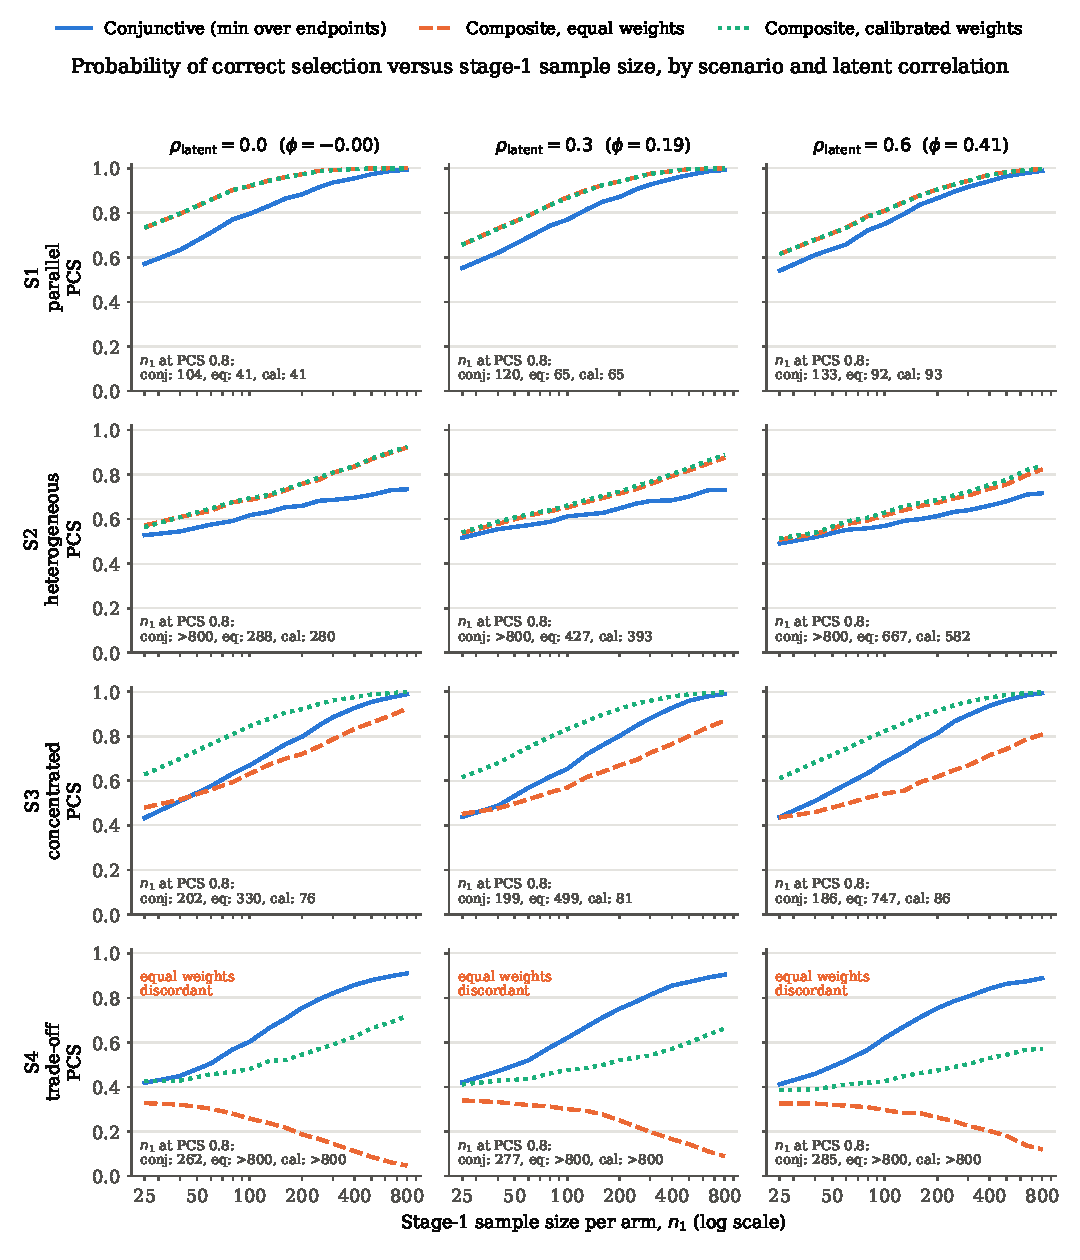
\includegraphics[width=\textwidth]{sim_fig.pdf}
\caption{Probability of correct selection against stage-1 sample size per arm, for the four configurations of Table~\ref{tab:scen} and three latent correlations. The horizontal line marks $\PCS^\ast=0.8$. In S4 the uniform-weight composite is discordant and its $\PCS$ decreases in $n_1$.}\label{fig:pcs}
\end{figure}

\begin{table}
\centering\footnotesize
\caption{Dependence on the number of doses, S1 parallel with adjacent dose effects spaced by 0.05, $\rho_{\mathrm{latent}}=0.3$, uniform weights. $\Delta N=(M-1)(n_1^{\mathrm{M}}-n_1^{\mathrm{C}})$ is the reduction in total sample size implied by \eqref{eq:accounting}.}\label{tab:msweep}
\begin{tabular}{ccccc}
\toprule
$M$ & $n_1^{\mathrm{M}}$ & $n_1^{\mathrm{C}}$ & Ratio & $\Delta N$ \\
\midrule
2 & 96 & 55 & 0.57 & 42 \\
3 & 118 & 63 & 0.54 & 108 \\
4 & 116 & 64 & 0.55 & 156 \\
5 & 115 & 62 & 0.54 & 212 \\
\bottomrule
\end{tabular}
\end{table}

Under parallel effects (S1) the composite gate needs 40--70\% of the conjunctive stage-1 size, and the observed ratio lies inside the bracket \eqref{eq:bracket} at each correlation; the saving diminishes as the endpoints become more strongly correlated, since the composite then averages less independent information. Under the heterogeneous plateau configuration (S2) the conjunctive gate does not reach the target within 800 subjects per arm, because the two leading doses are separated by only 0.01 on their binding endpoint, whereas the composite, which pools a separation of 0.0175 across endpoints with lower variance, reaches it at 280--580. Under the concentrated configuration (S3) uniform weights dilute the signal on endpoint 1 and the composite needs 1.6 to 4.0 times the conjunctive size, while calibrated weights, which load 0.85--0.95 on endpoint 1, reduce it to 0.38--0.46 of the conjunctive size. Under the trade-off configuration (S4) uniform weights are discordant and $\PCS$ falls with $n_1$; calibrated weights restore concordance but with a margin of at most about 0.01 on the composite scale, and the composite does not reach the target within the grid while the conjunctive gate does at 260--290. The ratio is stable in $M$ (Table~\ref{tab:msweep}) and the total reduction grows linearly with $M-1$, as \eqref{eq:accounting} implies.

\paragraph{Design rule (preliminary).}
On the selection-stage evidence alone, the composite gate is adopted only when, over the pre-specified scenario set $\Theta$, (i) $\bw^\star$ from \eqref{eq:weights} is concordant at every $\theta\in\Theta$, and (ii) simulation shows $n_1^{\mathrm{C}}(\bw^\star)<n_1^{\mathrm{M}}$ at the target $\PCS^\ast$ for the scenarios given positive prior weight. Section~\ref{sec:e2e} shows that condition (ii) is necessary but not sufficient and replaces it with a frontier criterion. If the conditions fail, the conjunctive gate is retained; the confirmatory analysis of Sections~\ref{sec:final} and \ref{sec:t1e} is unchanged in either case, since the error-control argument does not depend on the gate. The futility boundary $\eta$ is calibrated separately for whichever gate is used, so that the two designs are compared at equal probability of proceeding under the global null.


\subsection{End-to-end operating characteristics}\label{sec:e2e}

The selection-stage comparison of Section~\ref{sec:saving} is completed by simulating both designs through the interim gate, the futility rule, stage 2 and the final analysis. The reference design applies the co-primary criterion at both stages: doses are ranked by $\min_k z_{a,k}$ and the trial proceeds if $\min_k\Pr(p_{a^\star,k}-p_{C,k}>0\mid\bx^{(1)})\ge\eta$, as in Yang et al\cite{yang2024}. The proposed design ranks and gates on the composite. The final analysis is common: one-sided Wald $p$-values per endpoint and stage, Simes closure over doses on the stage-1 component, inverse-normal combination with $v_1=\sqrt{n_1/n_{\mathrm{tot}}}$, and the co-primary claim if and only if every endpoint is rejected at $\alpha=0.025$. The per-arm total on $a^\star$ and $C$ is fixed at $n_{\mathrm{tot}}=350$, so $n_2=n_{\mathrm{tot}}-n_1$ and sample size re-estimation is not used. The futility boundary $\eta$ is calibrated separately for each gate, weight vector and $n_1$ so that the probability of proceeding under the global null is $0.20$; the two designs are therefore compared at equal behaviour under $H_0$. Weights for the composite are uniform for S1 and S2 and, for S3 and S4, the vectors obtained at the selection stage at $\rho_{\mathrm{latent}}=0.3$, namely $\bw^\star(\mathrm{S3})=(0.95,0,0.05,0)$ and $\bw^\star(\mathrm{S4})=(0.20,0.25,0.05,0.50)$. Three null configurations are added: N0, the global null; N1, endpoint 4 null for every dose with endpoints 1--3 as in S1; and N2, doses 1 and 2 null with dose 3 as in S1. Each cell uses $10{,}000$ trials (Monte Carlo standard error at most $0.005$ for a probability, $0.0016$ for an error rate near $0.025$). Three runs are reported: (A) equal stage-1 cost, $n_1=100$ per arm; (B) equal selection accuracy, each design at its own $n_1$ from Table~\ref{tab:main}; and (C) the frontier of claim probability against expected total sample size as $n_1$ varies from 40 to 200, at $\rho_{\mathrm{latent}}=0.3$.

\begin{table}
\centering\footnotesize
\caption{Run A, equal stage-1 cost ($n_1=100$): probability of correct selection, probability of the co-primary claim (power) and expected total sample size, by design and latent correlation. False-claim rates in these configurations were at most $0.007$ (S3, where $\theta_{1,1}=0$).}\label{tab:e2eA}
\setlength{\tabcolsep}{3.5pt}
\begin{tabular}{llccccccccc}
\toprule
& & \multicolumn{3}{c}{$\rho_{\mathrm{lat}}=0$} & \multicolumn{3}{c}{$\rho_{\mathrm{lat}}=0.3$} & \multicolumn{3}{c}{$\rho_{\mathrm{lat}}=0.6$} \\
\cmidrule(lr){3-5}\cmidrule(lr){6-8}\cmidrule(lr){9-11}
Configuration & Design & PCS & Power & $E[N]$ & PCS & Power & $E[N]$ & PCS & Power & $E[N]$ \\
\midrule
S1 parallel & M: co-primary gate & 0.79 & 0.74 & 890 & 0.77 & 0.75 & 879 & 0.76 & 0.75 & 864 \\
 & C: composite, uniform $\mathbf w$ & 0.92 & 0.81 & 900 & 0.87 & 0.80 & 894 & 0.82 & 0.79 & 879 \\
\addlinespace[3pt]
S2 heterogeneous & M: co-primary gate & 0.61 & 0.49 & 883 & 0.61 & 0.54 & 866 & 0.59 & 0.55 & 847 \\
 & C: composite, uniform $\mathbf w$ & 0.69 & 0.52 & 899 & 0.65 & 0.55 & 892 & 0.63 & 0.57 & 877 \\
\addlinespace[3pt]
S3 concentrated & M: co-primary gate & 0.66 & 0.73 & 894 & 0.66 & 0.73 & 886 & 0.68 & 0.74 & 874 \\
 & C: composite, uniform $\mathbf w$ & 0.62 & 0.68 & 900 & 0.57 & 0.65 & 899 & 0.53 & 0.63 & 893 \\
 & C: composite, $\mathbf w^\star$(S3) & 0.83 & 0.71 & 806 & 0.83 & 0.72 & 809 & 0.82 & 0.72 & 801 \\
\addlinespace[3pt]
S4 trade-off & M: co-primary gate & 0.60 & 0.21 & 859 & 0.62 & 0.25 & 831 & 0.62 & 0.29 & 794 \\
 & C: composite, uniform $\mathbf w$ & 0.27 & 0.11 & 899 & 0.29 & 0.13 & 890 & 0.30 & 0.16 & 874 \\
 & C: composite, $\mathbf w^\star$(S4) & 0.47 & 0.18 & 875 & 0.46 & 0.22 & 847 & 0.44 & 0.24 & 820 \\
\bottomrule
\end{tabular}
\end{table}

\begin{table}
\centering\footnotesize
\caption{Run A, null configurations ($n_1=100$): probability of proceeding to stage 2 and probability of a false co-primary claim, by design and latent correlation. All false-claim rates are below $\alpha=0.025$.}\label{tab:e2eN}
\setlength{\tabcolsep}{4pt}
\begin{tabular}{llcccccc}
\toprule
& & \multicolumn{3}{c}{$\Pr(\text{proceed})$} & \multicolumn{3}{c}{$\Pr(\text{false claim})$} \\
\cmidrule(lr){3-5}\cmidrule(lr){6-8}
Configuration & Design & $\rho=0$ & $0.3$ & $0.6$ & $\rho=0$ & $0.3$ & $0.6$ \\
\midrule
N0 global null & M: co-primary gate & 0.21 & 0.21 & 0.21 & 0.0000 & 0.0000 & 0.0002 \\
 & C: composite, uniform $\mathbf w$ & 0.20 & 0.19 & 0.19 & 0.0000 & 0.0000 & 0.0002 \\
 & C: composite, $\mathbf w^\star$(S3) & 0.19 & 0.20 & 0.20 & 0.0000 & 0.0000 & 0.0001 \\
 & C: composite, $\mathbf w^\star$(S4) & 0.20 & 0.20 & 0.19 & 0.0000 & 0.0000 & 0.0003 \\
\addlinespace[3pt]
N1 endpoint-4 null & M: co-primary gate & 0.71 & 0.63 & 0.55 & 0.0103 & 0.0128 & 0.0165 \\
 & C: composite, uniform $\mathbf w$ & 0.98 & 0.93 & 0.85 & 0.0135 & 0.0161 & 0.0142 \\
 & C: composite, $\mathbf w^\star$(S3) & 0.87 & 0.87 & 0.86 & 0.0095 & 0.0127 & 0.0156 \\
 & C: composite, $\mathbf w^\star$(S4) & 0.76 & 0.68 & 0.61 & 0.0140 & 0.0178 & 0.0169 \\
\addlinespace[3pt]
N2 doses 1-2 null & M: co-primary gate & 0.95 & 0.93 & 0.89 & 0.0000 & 0.0000 & 0.0000 \\
 & C: composite, uniform $\mathbf w$ & 1.00 & 0.98 & 0.93 & 0.0000 & 0.0000 & 0.0000 \\
 & C: composite, $\mathbf w^\star$(S3) & 0.82 & 0.82 & 0.81 & 0.0000 & 0.0000 & 0.0000 \\
 & C: composite, $\mathbf w^\star$(S4) & 0.99 & 0.96 & 0.92 & 0.0000 & 0.0000 & 0.0000 \\
\bottomrule
\end{tabular}
\end{table}

\begin{table}
\centering\footnotesize
\caption{Run B, equal selection accuracy: each design at the $n_1$ giving $\PCS=0.8$ at the selection stage (Table~\ref{tab:main}).}\label{tab:e2eB}
\begin{tabular}{llcccccc}
\toprule
Configuration & $\rho_{\mathrm{lat}}$ & Design & $n_1$ & $\Pr(\text{proceed})$ & PCS & Power & $E[N]$ \\
\midrule
S1 parallel & 0.0 & M: co-primary gate & 104 & 0.982 & 0.802 & 0.744 & 899 \\
 & 0.0 & C: composite, uniform $\mathbf w$ & 41 & 0.947 & 0.802 & 0.733 & 749 \\
 & 0.3 & M: co-primary gate & 120 & 0.974 & 0.807 & 0.776 & 928 \\
 & 0.3 & C: composite, uniform $\mathbf w$ & 65 & 0.944 & 0.814 & 0.758 & 798 \\
 & 0.6 & M: co-primary gate & 133 & 0.963 & 0.801 & 0.795 & 950 \\
 & 0.6 & C: composite, uniform $\mathbf w$ & 92 & 0.945 & 0.804 & 0.778 & 856 \\
\addlinespace[3pt]
S3 concentrated & 0.0 & M: co-primary gate & 202 & 0.999 & 0.804 & 0.838 & 1104 \\
 & 0.0 & C: composite, $\mathbf w^\star$(S3) & 76 & 0.735 & 0.792 & 0.636 & 707 \\
 & 0.3 & M: co-primary gate & 199 & 0.997 & 0.800 & 0.836 & 1097 \\
 & 0.3 & C: composite, $\mathbf w^\star$(S3) & 81 & 0.754 & 0.802 & 0.656 & 730 \\
 & 0.6 & M: co-primary gate & 186 & 0.992 & 0.807 & 0.840 & 1069 \\
 & 0.6 & C: composite, $\mathbf w^\star$(S3) & 86 & 0.767 & 0.795 & 0.673 & 749 \\
\bottomrule
\end{tabular}
\end{table}

\begin{table}
\centering\footnotesize
\caption{Run C, frontier in $n_1$ at $\rho_{\mathrm{latent}}=0.3$: co-primary gate (M) against the composite gate (C; uniform weights in S1, $\bw^\star(\mathrm{S3})$ in S3).}\label{tab:e2eC}
\begin{tabular}{lccccccc}
\toprule
& & \multicolumn{3}{c}{M: co-primary gate} & \multicolumn{3}{c}{C: composite gate} \\
\cmidrule(lr){3-5}\cmidrule(lr){6-8}
Configuration & $n_1$ & PCS & Power & $E[N]$ & PCS & Power & $E[N]$ \\
\midrule
S1 parallel & 40 & 0.636 & 0.604 & 697 & 0.727 & 0.645 & 687 \\
 & 60 & 0.692 & 0.654 & 748 & 0.791 & 0.740 & 781 \\
 & 80 & 0.746 & 0.716 & 821 & 0.836 & 0.784 & 843 \\
 & 100 & 0.782 & 0.747 & 880 & 0.869 & 0.803 & 894 \\
 & 120 & 0.800 & 0.771 & 928 & 0.894 & 0.821 & 938 \\
 & 150 & 0.841 & 0.789 & 996 & 0.914 & 0.827 & 1000 \\
 & 200 & 0.876 & 0.815 & 1099 & 0.945 & 0.829 & 1100 \\
\addlinespace[3pt]
S3 concentrated & 40 & 0.505 & 0.573 & 722 & 0.683 & 0.460 & 509 \\
 & 60 & 0.556 & 0.614 & 772 & 0.750 & 0.572 & 627 \\
 & 80 & 0.620 & 0.683 & 833 & 0.798 & 0.659 & 726 \\
 & 100 & 0.661 & 0.732 & 887 & 0.821 & 0.720 & 807 \\
 & 120 & 0.707 & 0.766 & 931 & 0.853 & 0.759 & 872 \\
 & 150 & 0.753 & 0.803 & 997 & 0.885 & 0.815 & 964 \\
 & 200 & 0.806 & 0.840 & 1099 & 0.912 & 0.862 & 1087 \\
\bottomrule
\end{tabular}
\end{table}

\begin{figure}
\centering
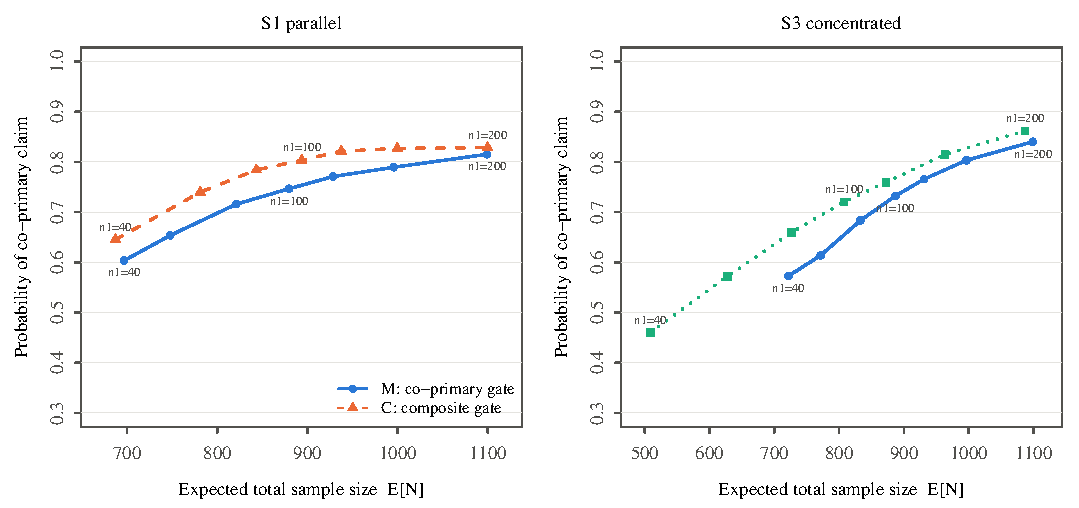
\includegraphics[width=\textwidth]{sim_e2e_fig.pdf}
\caption{Run C: probability of the co-primary claim against expected total sample size as $n_1$ varies from 40 to 200 per arm ($\rho_{\mathrm{latent}}=0.3$, $n_{\mathrm{tot}}=350$). A curve lying above and to the left dominates.}\label{fig:frontier}
\end{figure}

\paragraph{Error control.}
In every null configuration and for every design the false-claim rate is below $0.025$ (Table~\ref{tab:e2eN}), as the proposition of Section~\ref{sec:t1e} requires; the selection functional does not affect it. Under the global null the intersection--union claim is very conservative (at most $0.0003$), since four null endpoints must all be rejected. The configuration that exercises the bound is N1, a single null endpoint with strong effects elsewhere, where the rates are $0.010$--$0.018$; the residual conservatism comes from the Simes closure and the futility rule.

\paragraph{Equal cost (run A).}
Where the composite carries more dose-discriminating information than the binding endpoint, the advantage at the selection stage carries through to the claim. In S1 the composite gate raises PCS from $0.76$--$0.79$ to $0.82$--$0.92$ and power from $0.74$--$0.75$ to $0.79$--$0.81$ at essentially the same $E[N]$; in S2 the gains are smaller but in the same direction. In S3 uniform weights lose on both PCS and power, while $\bw^\star(\mathrm{S3})$ raises PCS from $0.66$--$0.68$ to $0.82$--$0.83$ and matches the reference power ($0.71$--$0.72$ against $0.73$--$0.74$) with $E[N]$ lower by about ten per cent, the difference in $E[N]$ arising because the composite gate, which is here nearly a single-endpoint gate, proceeds in $80$--$82$\% of trials against $95$--$99$\% for the co-primary gate, whose go decision benefits from the large effects on endpoints 2--4. In S4 the reference design is better on every measure, with uniform weights discordant and calibrated weights concordant by too small a margin.

\paragraph{Equal selection accuracy (run B).}
Matching $n_1$ to $\PCS=0.8$ gives, in S1, an $E[N]$ lower by $10$--$17$\% at a power lower by $0.01$--$0.02$; the stage-1 saving is realised almost in full. In S3 the composite reaches $\PCS=0.8$ at $n_1\approx80$, but at that size the null-calibrated futility rule stops an effective drug in $23$--$27$\% of trials and the weak stage-1 component of the combination test costs further power, so $E[N]$ is lower by $30$--$36$\% but power falls from $0.84$ to $0.64$--$0.67$. Equal selection accuracy is therefore not the right basis for choosing $n_1$: the stage-1 size also governs the futility decision and the stage-1 contribution to the confirmatory test.

\paragraph{Frontier (run C).}
Figure~\ref{fig:frontier} and Table~\ref{tab:e2eC} trace both designs as $n_1$ varies. Read row by row, at equal $n_1$, Table~\ref{tab:e2eC} shows the composite design with a slightly higher $E[N]$ in S1 ($894$ against $880$ at $n_1=100$). This is the futility rule: both gates proceed in $20$\% of trials under the global null, and under the alternative the composite then proceeds more often ($0.987$ against $0.960$ at $n_1=100$), so it spends the stage-2 sample more often. Since $E[N]=(M+1)n_1+2n_2\Pr(\text{proceed})$, fewer false futility stops raise $E[N]$ at fixed $n_1$; the same mechanism is part of the composite's power advantage at equal $n_1$. In S3 the sign reverses ($807$ against $887$), the near-single-endpoint composite proceeding less often. The comparison that matters is at equal power, and Table~\ref{tab:e2eCm} interpolates each frontier at fixed power targets. In S1 the composite reaches the same claim probability with $7$--$15$\% fewer expected subjects, the saving growing with the target because the co-primary gate's curve flattens: power $0.80$ needs $n_1=171$ and $E[N]=1038$ under the co-primary gate against $n_1=96$ and $E[N]=885$ under the composite. In S3 the saving is $5$--$11$\%, and the composite reaches each target at a similar $n_1$ but lower $E[N]$, because it stops more often. The S3 saving is well below the selection-stage ratio of about $0.4$: with $n_{\mathrm{tot}}$ fixed, the stage-1 saving is diluted by the confirmatory sample, and a single-endpoint composite gives a less decisive futility decision than a conjunctive gate when every endpoint responds.

\begin{table}
\centering\footnotesize
\caption{Run C at matched power: stage-1 size and expected total sample size needed to reach a target claim probability, by linear interpolation of the frontiers in Table~\ref{tab:e2eC} ($\rho_{\mathrm{latent}}=0.3$).}\label{tab:e2eCm}
\begin{tabular}{lcccccc}
\toprule
& & \multicolumn{2}{c}{M: co-primary gate} & \multicolumn{2}{c}{C: composite gate} & \\
\cmidrule(lr){3-4}\cmidrule(lr){5-6}
Configuration & Target power & $n_1$ & $E[N]$ & $n_1$ & $E[N]$ & $E[N]$ ratio C/M \\
\midrule
S1 parallel & 0.65 & 59 & 744 & 41 & 692 & 0.93 \\
 & 0.70 & 75 & 802 & 52 & 742 & 0.92 \\
 & 0.75 & 103 & 887 & 65 & 795 & 0.90 \\
 & 0.80 & 171 & 1038 & 96 & 885 & 0.85 \\
\addlinespace[3pt]
S3 concentrated & 0.65 & 70 & 804 & 78 & 716 & 0.89 \\
 & 0.70 & 87 & 851 & 93 & 780 & 0.92 \\
 & 0.75 & 111 & 910 & 115 & 857 & 0.94 \\
 & 0.80 & 147 & 991 & 142 & 939 & 0.95 \\
\bottomrule
\end{tabular}
\end{table}

\paragraph{Futility behaviour under a single null endpoint.}
Under N1 the co-primary gate proceeds in $55$--$71$\% of trials, the uniform composite in $85$--$98$\%. A composite averages a null component with three positive ones and does not register the failure; the conjunctive gate does. The final analysis protects the error rate in both cases, but the composite design spends the stage-2 sample far more often when one component is inert ($E[N]$ of $827$--$889$ against $677$--$757$). This is the price of the composite gate, and it should be weighed against the selection advantage in any setting where failure on a single component is a realistic outcome.

\paragraph{Revised design rule.}
The stage-1 size is chosen from the frontier, not from selection accuracy alone: for the pre-specified $\Theta$, $\bw^\star$ from \eqref{eq:weights} must be concordant at every $\theta\in\Theta$; $\eta$ is calibrated under the global null; and $n_1$ is the smallest value at which the composite design attains the target claim probability, with the composite adopted only if its $E[N]$ at that point is below that of the co-primary gate at its own smallest adequate $n_1$. Where the scenario set gives material weight to single-component failure, the expected sample size under that configuration enters the comparison as well.

\subsection{Further operating characteristics}

Beyond the quantities reported above, the full evaluation covers cell configurations with identical marginals and pairwise dependence but differing higher-order cell mass, since these move the conjunction probability; expected duration; bias and coverage of the pooled and stage-2-only estimates for the selected dose; sample size re-estimation by \eqref{eq:ppos}; and sensitivity to $\bw$, to the prior $\balpha_a$, and to mis-specification of the scenario set $\Theta$.
